\documentclass[conference]{IEEEtran}
\IEEEoverridecommandlockouts
% The preceding line is only needed to identify funding in the first footnote. If that is unneeded, please comment it out.
\usepackage{cite}
\usepackage{amsmath,amssymb,amsfonts}
\usepackage{algorithmic}
\usepackage{graphicx}
\usepackage{tikz}\usetikzlibrary{arrows.meta,backgrounds,fit,positioning,shapes.geometric}
\usepackage{textcomp}
\usepackage{xcolor}
\usepackage{fancyhdr}
\usepackage{hyperref}
\usepackage{booktabs}
\usepackage{makecell}
\usepackage{amsthm}
\theoremstyle{plain}
\newtheorem{observation}{Observation}
% Allow slightly looser inter-word spacing so that long identifiers and
% hyphenated terms do not push a line past the column edge.
\setlength{\emergencystretch}{1.2em}

\def\BibTeX{{\rm B\kern-.05em{\sc i\kern-.025em b}\kern-.08em
    T\kern-.1667em\lower.7ex\hbox{E}\kern-.125emX}}

\fancypagestyle{firstpage}{
  \fancyhf{} % Clear header and footer
  \fancyhead[C]{23rd Edition of IEEE India Council International Conference (INDICON 2026)}
  \fancyfoot[L]{%
      \begin{minipage}[t]{\textwidth}
      \normalsize{979-8-3195-2581-9/26/\$31.00 \copyright2026 IEEE}
    \end{minipage}%
  }
  \renewcommand{\headrulewidth}{0pt} % Remove the horizontal line
}

\pagestyle{fancy}
\fancyhf{} % Clear the default header and footer
\fancyfoot[C]{INDICON 2026}
\renewcommand{\headrulewidth}{0pt} % Remove the horizontal line



\begin{document}


\title{Intent-Adaptive Hybrid Retrieval and Heterogeneous-Space Person Fusion for Conversational Video Surveillance}

\author{
\IEEEauthorblockN{Sujal M H\textsuperscript{1,*}, Sujnan Kumar\textsuperscript{1}, Yashas Shetty\textsuperscript{1}, Suhan D Shet\textsuperscript{1}, and Ravinarayana B\textsuperscript{2}}
\IEEEauthorblockA{\textit{Department of Computer Science and Engineering}\\
\textit{Mangalore Institute of Technology and Engineering}\\
Moodabidre, India\\
Email: \{sujalmh9, sujankumar439, yashass825, suhanshet2004\}@gmail.com, hodcse@mite.ac.in}
\IEEEauthorblockA{\textit{Head, Department of Computer Science and Engineering}\\
\textit{Mangalore Institute of Technology and Engineering}\\
Moodabidre, India}
\textsuperscript{*}Corresponding author
}

\maketitle
\thispagestyle{firstpage}

\begin{abstract}
\sloppy
Conversational surveillance requires turning free text into executable alert rules, representing people across visual and attribute spaces, and ranking candidates from structured and semantic branches. We present an integrated system that couples these decisions in one pipeline and evaluate it on a four-camera deployment and a released single-camera reproducibility track. The system combines a deterministic, schema-validated 9-tuple alert compiler with clarify/abstain validation (30/30 clean and 30/30 stress on the released benchmark, no false materializations); a heterogeneous SigLIP+MiniLM person descriptor that improves P@5 over visual-only and RRF on the released track (0.427 vs.\ 0.407 and 0.361); and a training-free intent-adaptive routing rule that matches the best tune-selected fixed alpha (0.538 vs.\ 0.538) and ties it end-to-end (0.450 vs.\ 0.448), removing the need for a per-site alpha sweep. The deployment study provides the motivating measurements; the released track makes the pipeline re-computable. The system is released with its benchmark definitions and measured outputs.
\fussy
\end{abstract}

\begin{IEEEkeywords}
Conversational Alert Authoring, Person Descriptor Retrieval, Heterogeneous Embedding Fusion, Hybrid Retrieval, Intent-Adaptive Ranking, Vision--Language Surveillance.
\end{IEEEkeywords}

\section{Introduction}

\IEEEPARstart{N}{atural}-language interfaces over surveillance video are feasible: instance segmentation, person descriptor retrieval and contrastive vision--language models are mature, and structured-output LLMs turn an utterance into a typed query schema. The unsolved problem is \emph{how to rank} candidate frames: a structured filter (\textit{``persons in Zone~A between 22:00 and 23:00''}) and a semantic vector lookup (\textit{``red jacket loitering near the entrance''}) give two incommensurable scales. Dominant fusion strategies: a fixed convex sum $\alpha S_{\text{struct}} + (1-\alpha) S_{\text{sem}}$ tuned once per system~\cite{b7,b12,b29}, parameter-free Reciprocal Rank Fusion~\cite{b27}, or sequential filter-then-rank pipelines~\cite{b30}. On the released protocol-matched control the best tune-selected fixed $\alpha$ reaches 0.538 macro-mean P@5 and the training-free adaptive rule matches it at 0.538, removing the need for a per-site $\alpha$ sweep; the four-camera deployment recorded larger absolute gains, reported in the deployment study table.

Two gaps compound this: hand-translation of behavior into typed rules, and same-space-only descriptor fusion needing matched backbones deployments rarely have.

\subsection*{Contributions}
\begin{enumerate}
\item \textbf{An integrated conversational surveillance system.} One query schema couples alert authoring, heterogeneous person descriptor retrieval and adaptive hybrid retrieval; the paper reports a four-camera deployment study and releases a single-camera reproducibility track with code, benchmark definitions and measured outputs.
\item \textbf{A deterministic, schema-validated alert compiler.} Nine-field rules with clarify/abstain; released test split 30/30 clean and 30/30 stress with zero false materializations; fuzz and adversarial probes. The deployment study used an LLM-backed materializer and is reported in the deployment table.
\item \textbf{A heterogeneous person descriptor with a fair comparison.} SigLIP+MiniLM concatenation gives P@5 0.427 vs.\ 0.407 visual-only and 0.361 RRF on the released track; zero-pad/norm-matched and learned projection are statistically indistinguishable, so the gain comes from combining views rather than the specific concatenation operator. No identity claim.
\item \textbf{A training-free intent-adaptive routing rule.} Matches the best tune-selected fixed alpha (0.538 = 0.538) and ties end-to-end (0.450 vs.\ 0.448), removing the need for a per-site alpha sweep. The four-camera deployment recorded the larger gains in the deployment table; the released track is the reproducibility check.
\end{enumerate}

\section{Related Work and Position}

We compare with the closest published work along the three axes below. To our knowledge, no prior system couples conversational alert authoring, heterogeneous frozen-encoder person descriptors and adaptive hybrid retrieval, and reports a deployment study alongside a released reproducibility track.

\textbf{Conversational alert authoring.} Form-driven editors and slot-filling LLMs are standard; the contribution is reusing the same query-parsing schema to materialize a 9-tuple rule end-to-end.

\textbf{Multimodal person Re-ID.} Heterogeneous-dimensional concatenation of frozen encoders is an IR retrieval pattern; we evaluate it as the \emph{primary} surveillance-Re-ID descriptor. Prior NL-based person-search~\cite{b32} couples a dual encoder by joint training or descriptive fusion over same-dimensional modalities; rank-based late fusion~\cite{b27} needs two indices and score normalization. To our knowledge, no deployed Re-ID system uses heterogeneous weighted concatenation as a single FAISS index calibrated on 50 pairs. A 2025 survey of text-based person Re-ID taxonomizes evaluation, strategy, architecture and optimization over established attribute-to-language retrieval designs~\cite{b36}; our construction differs in fusing frozen, dimensionally-mismatched encoders with no joint training as a single FAISS index.

\textbf{Hybrid structured/semantic retrieval.} Dense plus structured retrieval is established IR practice~\cite{b25,b27,b29}, mainly via fixed-$\alpha$ convex combination or parameter-free RRF~\cite{b27}; convex-combination analysis finds the learned blend sample-efficient and normalization-agnostic, beating RRF in- and out-of-domain~\cite{b33}. IR query-dependent weighting learns weights from click data without hard overrides; per-query $\alpha$ predictors~\cite{b34} need training data or per-query LLM scoring, unlike our training-free rule. Override-routing with category hard overrides plus heterogeneous single-index fusion is undemonstrated for surveillance video to our knowledge.

\section{Background and System Substrate}

The nine-model near-real-time pipeline runs capture, perception, indexing, reasoning and output layers; all but C1--C3 are off-the-shelf. Live 1080p streams (2~FPS) pass YOLOv11m-seg~\cite{b14}, OSNet $x1\_0$ tracking~\cite{b22b}, PAR-crossroad-0238 attributes and CIEDE2000 colour naming into two FAISS \texttt{IndexFlatIP} indices~\cite{b25}: scene embeddings ($\mathbb{R}^{512}$, OpenCLIP ViT-B/32~\cite{b18b}) and person descriptors ($\mathbb{R}^{1152}$, \S\ref{sec:fusion}); MongoDB holds 12 compound-indexed collections. Captions come from a tiered VLM pipeline; the NL parser is a structured-output LLM. Fig.~\ref{fig:system} summarizes the dataflow.

\begin{figure}[!t]
\centering
% Figure 1 — system dataflow for INDICON 850.
% Input this file inside a figure environment (see area report for the block).
% Self-contained: needs \usepackage{tikz} and
% \usetikzlibrary{arrows.meta,backgrounds,fit,positioning,shapes.geometric} in the preamble.
% Scales itself to \columnwidth so the 6-page budget is preserved.
\resizebox{\columnwidth}{!}{%
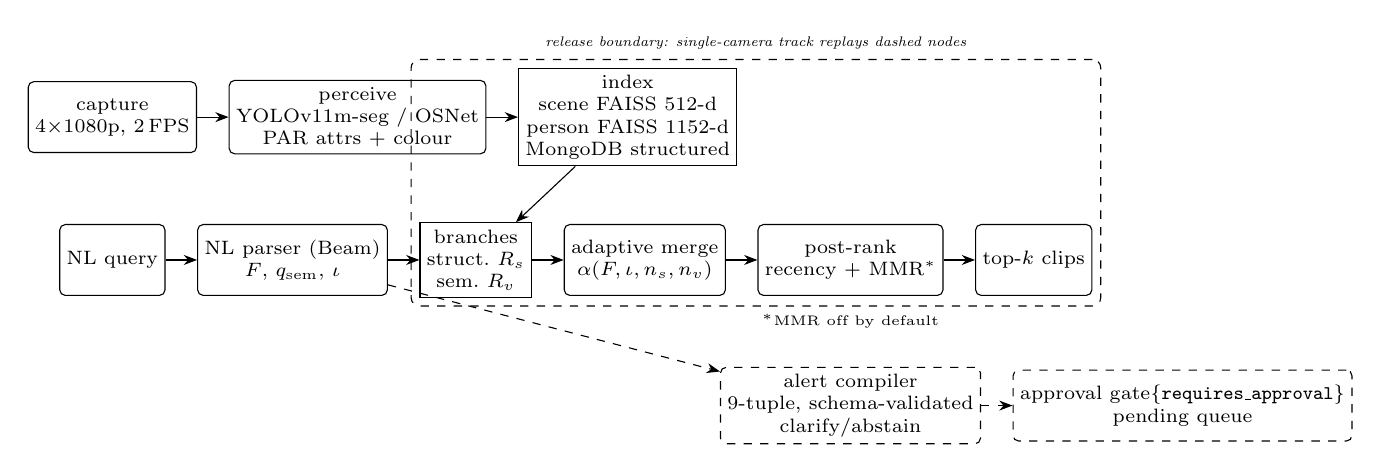
\begin{tikzpicture}[
  node distance=4mm,
  font=\scriptsize,
  >=Stealth,
  box/.style={draw, rounded corners=2pt, align=center, inner sep=2.5pt, minimum height=9mm},
  data/.style={draw, align=center, inner sep=2.5pt, minimum height=9mm},
  lbl/.style={font=\tiny, align=center},
]
% --- Lane 1: capture / perceive / index ---
\node[box] (cap) {capture\\4$\times$1080p, 2\,FPS};
\node[box, right=of cap] (per) {perceive\\YOLOv11m-seg / OSNet\\PAR attrs + colour};
\node[data, right=of per] (idx) {index\\scene FAISS 512-d\\person FAISS 1152-d\\MongoDB structured};
% --- Lane 2: query / retrieve / rank ---
\node[box, below=9mm of cap] (qry) {NL query};
\node[box, right=of qry] (prs) {NL parser (Beam)\\$F$, $q_{\mathrm{sem}}$, $\iota$};
\node[data, right=of prs] (br) {branches\\struct.\ $R_s$\\sem.\ $R_v$};
\node[box, right=of br] (mrg) {adaptive merge\\$\alpha(F,\iota,n_s,n_v)$};
\node[box, right=of mrg] (prk) {post-rank\\recency + MMR$^*$};
\node[box, right=of prk] (top) {top-$k$ clips};
% --- Side: alert compiler + approval gate ---
\node[box, dashed, below=9mm of prk] (alr) {alert compiler\\9-tuple, schema-validated\\clarify/abstain};
\node[box, dashed, right=of alr] (apv) {approval gate\{\tt requires\_approval\}\\pending queue};
% --- Arrows ---
\draw[->] (cap) -- (per);
\draw[->] (per) -- (idx);
\draw[->] (idx) -- (br);
\draw[->] (qry) -- (prs);
\draw[->] (prs) -- (br);
\draw[->] (br) -- (mrg);
\draw[->] (mrg) -- (prk);
\draw[->] (prk) -- (top);
\draw[->, dashed] (prs) -- (alr);
\draw[->, dashed] (alr) -- (apv);
\node[lbl, below=1mm of prk] {$^*$MMR off by default};
% --- Release boundary: dashed fit around the replayed nodes ---
\begin{scope}[on background layer]
\node[draw, dashed, rounded corners=3pt, inner sep=3pt,
  fit=(idx) (br) (mrg) (prk) (top),
  label={{[font=\tiny\itshape]above:release boundary: single-camera track replays dashed nodes}}] {};	
\end{scope}
\end{tikzpicture}%
}

\caption{System dataflow. Capture feeds perception (YOLOv11m-seg, OSNet, PAR
attributes, colour) into scene/person FAISS indices and MongoDB. The NL parser
(Beam) emits filter $F$, semantic query $q_{\mathrm{sem}}$ and intent $\iota$;
structured ($R_s$) and semantic ($R_v$) branches merge with the adaptive weight
$\alpha(F,\iota,n_s,n_v)$, then post-ranking (recency; MMR off by default)
returns top-$k$ clips. The schema-validated alert compiler plus the
\texttt{requires\_approval} gate stage consequential alerts in a pending queue.
Dashed nodes replay in the released single-camera reproducibility track.}
\label{fig:system}
\end{figure}

\section{C1: Conversational Alert Compiler}\label{sec:alert_grammar}

\paragraph*{Grammar}
A typed alert rule is the 9-tuple $\mathcal{R} = \langle\, e,\mathcal{O},\zeta,\tau,\mathcal{T},s,c,\Sigma,\kappa\,\rangle$ with event $e$, objects $\mathcal{O}$, zone $\zeta$, threshold $\tau$, time window $\mathcal{T}$ (cross-midnight), severity $s$ (default \texttt{info}), cooldown $c$ in seconds (default $60$), side-effects $\Sigma$ and cadence $\kappa$ in Hz (default $1$), reducing manual rule authoring to a clarification round-trip. The \emph{released} NL-to-rule materializer is a deterministic keyword/regex module (\texttt{alert\_\allowbreak materializer.py}: intents, event/time keywords, $\tau$/cooldown numbers, clarify/abstain classification), not LLM structured-output. On the released author-constructed benchmark it materializes all 30 clean test utterances with nine exactly correct fields and clarifies all 30 stress test utterances, with zero false materializations (\texttt{results/alert\_results.md}); the deployment study with the LLM-backed materializer is reported in the deployment study table (\S\ref{sec:eval}); the two paths are complementary, not interchangeable.

\paragraph*{Authoring example}
The utterance \textit{``alert me when more than five people gather in Zone~A after 10~PM''} produces $\mathcal{R} = \langle\text{crowd},\{\text{person}\},\text{Zone~A},({>},5),[22{:}00,06{:}00],\allowbreak\text{info},60,\{\text{snapshot},\text{push\_ws}\},1\text{Hz}\rangle$
without manual configuration: unstated severity, cooldown, side-effects and cadence take defaults. Six rule families run per frame---crowd, loitering ($\Delta t{\ge}60$~s), fight ($\bar{\mathcal{E}}_W{\ge}0.03$, centres $<24$~px), zone occupancy, count and time-of-day (cross-midnight)---each cached from MongoDB with a 5-second TTL. Ambiguous cases (fuzzy zone, implicit ``a few'', cross-midnight) clarify rather than materialize.

\paragraph*{Validation safeguards (clarify/abstain)}
Unknown zones, missing thresholds or time windows, and unsupported verbs (e.g., ``follow him home'', ``identify the person'') trigger schema validation requesting clarification, not a rule. Stress-kind classification and 9-tuple validation are deterministic and tested (\texttt{backend/\allowbreak tests/\allowbreak test\_\allowbreak alerts.py}). A minimal-question policy asks only required slots without documented defaults, in dependency order (\texttt{clarification\_\allowbreak policy.py}). Conjunctive bounds combine into one threshold, zone aliases are masked before the object scan, and any rule the validator rejects is clarified rather than reported clean. Two-zone conjunctions clarify naming both zones, `until/till' times materialize a midnight-to-hour window, invalid clock times clarify, and a 215-case adversarial set holds at zero silent drops.

\paragraph*{Release probes} The deterministic compiler with the schema-validated clarify/abstain check scores 30/30 clean test rules fully correct and 30/30 stress test utterances clarified, with zero false materializations and clarify precision/recall/F1 of 1.000/1.000/1.000. Coverage probes extend this: compositional held-out over one (event,zone) combo per event (9/9 held-out vs.\ 51/51 seen rule-correct), a simulated-oracle dialogue (90 seeded episodes) at 1.08 mean turns vs.\ 2.58 for a naive per-field baseline with 90/90 rules valid, seeded fuzz (2{,}000 noise utterances plus 200 unsupported-hint cases) with zero crashes, zero soundness violations and zero false materializations, and a grammar-aware adversarial round (20{,}000 fuzz inputs, 38 reproducers) with zero residual violations and all 14 shipped invariants intact (\texttt{eval\_\allowbreak alerts.py}, \texttt{results/c3probe2\_report.md}).

\paragraph*{Statistical anomaly complement} A rolling 7-day per-(camera,hour) baseline emits events on large Z-scores; F$_1$ reaches $0.840$/$0.834$/$0.751$ on a 7-day labeled subset.

\section{C2: Heterogeneous-Space Person Fusion}\label{sec:fusion}

\paragraph*{Problem}
Person descriptor retrieval across heterogeneous spaces must use the
encoders at hand---here SigLIP-base ($\mathbb{R}^{768}$)~\cite{b24} and
MiniLM-L12-v2 ($\mathbb{R}^{384}$)~\cite{b23}, of differing dimensionality.
We evaluate retrieval over metadata-formed pseudo-tracks, not identities.

\paragraph*{Construction}
Per person ROI we form
\begin{align}
\mathbf{v} &= \mathrm{SigLIP}(\mathrm{Mask}(\mathrm{ROI})) \in\mathbb{R}^{768},\ \text{L2-normalized} \notag\\
\mathbf{t} &= \mathrm{MiniLM}\bigl(\mathrm{Text}(\hat{y}, C)\bigr) \in\mathbb{R}^{384},\ \text{L2-normalized},
\end{align}
where $\mathrm{Text}(\hat{y}, C)$ is the sentence from the seven sigmoid predictions and the color. Text-only search ($\mathbf{v}{=}\mathbf{0}$) ranks by text cosine, so the gains do not come from it. Person gallery (deployment): full four-camera gallery; deployment calibration uses a held-out 50-pair split. Released track: $N{=}1{,}778$ descriptors, 280 metadata-formed pseudo-tracks (210 test~/~70 calibration), 1{,}190 test queries; 1{,}008 calibration pairs (504\texttt{+}/504\texttt{-}) with whole-track 5-fold CV.
\begin{equation}
\mathbf{e}_{\text{fused}} = \frac{[\,\alpha_v\,\mathbf{v}\;\Vert\;\beta_t\,\mathbf{t}\,]}{\bigl\Vert [\,\alpha_v\,\mathbf{v}\;\Vert\;\beta_t\,\mathbf{t}\,]\bigr\Vert_2}\;\in\mathbb{R}^{1152},
\label{eq:fusion}
\end{equation}
with $(\alpha_v,\beta_t)=(0.6, 0.4)$ from a coarse grid search on the unit simplex (step $0.1$, nine pairs) maximizing F$_{5,10}$ on the held-out calibration set, where F$_{5,10}$ $\triangleq$ H-mean(P@5,R@10). Both branches enter unit-norm, so $\Vert[0.6\mathbf{v}\,\Vert\,0.4\mathbf{t}]\Vert_2^2{=}0.52$ and the fused cosine is $(0.36\cos_v{+}0.16\cos_t)/0.52$: the effective block weights are $9/13{\approx}0.69$ visual and $4/13{\approx}0.31$ text, not $0.6/0.4$.

\paragraph*{Why concatenation, not addition}
Same-space addition needs a projection $\mathbf{P}\in\mathbb{R}^{768\times 384}$ and is norm-sensitive; weighted concatenation preserves both encoders' rank, needs no joint training, and learns only $(\alpha_v,\beta_t)$.

\paragraph*{Ablation}
The released track is the primary comparison; the deployment is a recorded observation stated once below and in the deployment study table.

\begin{table}[!t]
\caption{Released single-camera person-descriptor track (shipped original-index measurement); metadata-formed pseudo-tracks (280 tracks, 1{,}190 queries, 1{,}778 descriptors), not identities. Paired bootstrap, 3{,}000 resamples; Holm over competitors. Concat beats visual ($\Delta{+}0.021$, $p{<}0.0007$) and RRF ($\Delta{+}0.067$, $p{<}0.0007$); zero-pad and learned projection tie; gated is $+$0.017 P@5 at pair-AUC parity.}
\label{tab:fusion_ablation}
\centering
\footnotesize
\begin{tabular}{@{}lcccc@{}}
\toprule
Method & P@5 & R@10 & F$_{5,10}$ & 95\% CI \\
\midrule
Visual only & 0.407 & 0.285 & 0.290 & [0.390,0.424] \\
Text only & 0.102 & 0.095 & 0.077 & [0.089,0.116] \\
\textbf{Concat (ours)} & \textbf{0.427} & \textbf{0.311} & \textbf{0.309} & \textbf{[0.410,0.445]} \\
Zero-pad~/~norm-matched & 0.428 & 0.312 & 0.309 & [0.410,0.446] \\
Learned projection & 0.432 & 0.311 & 0.312 & [0.415,0.450] \\
5-seed random projection & 0.417 $\pm{<}0.001$ & 0.297 & 0.298 & seeds \\
RRF & 0.361 & 0.285 & 0.266 & [0.343,0.378] \\
Gated rank (post-hoc) & 0.444 & 0.307 & 0.315 & [0.425,0.462] \\
\bottomrule
\end{tabular}
\end{table}

Concat beats visual-only ($\Delta{+}0.021$, Holm $p{<}0.0007$) and RRF ($\Delta{+}0.067$, Holm $p{<}0.0007$); zero-pad/norm-matched ($\Delta{+}0.001$, Holm $p{=}0.69$) and learned projection ($\Delta{+}0.005$, Holm $p{=}0.21$) tie with concat, while gated rank is $+$0.017 P@5 (Holm $p{=}0.0053$) at pair-AUC parity (Holm $p{=}0.98$). The tie shows the gain comes from combining views, not the concatenation operator; no identity claim is made. The metadata-only track keeps concat first but puts visual above RRF (0.427/0.407/0.361); the visual-cosine formation is kept only as a biased sensitivity slice, which is why formation is fixed to metadata. The four-camera deployment recorded a larger two-view gain (deployment study table); it is not part of this table.

\section{C3: Intent-Adaptive Routing Rule}\label{sec:adaptive_alpha}

\paragraph*{Problem}
A natural-language query $q$ is parsed into a structured filter $F$ (14 typed fields, incl.\ \texttt{action}) and a semantic payload $q_{\text{sem}}$. Structured branch: $R_s=\{r\}$ from MongoDB with $S_{\text{struct}}(r)\in[0,1]$ (duration max-scaled per query); semantic branch: $R_v$ from FAISS with per-query min-max normalized $S_{\text{sem}}(r)\in[0,1]$ (\texttt{score\_norm}). The hybrid score is the convex combination
\begin{equation}
S_{\text{hyb}}(r) = \alpha\, S_{\text{struct}}(r) + (1-\alpha)\, S_{\text{sem}}(r),\quad \alpha\in[0,1].
\label{eq:hybrid_score}
\end{equation}

\paragraph*{Fixed-\texorpdfstring{$\alpha$}{alpha} baselines (released control)}
We sweep $\alpha\in\{0.0,\allowbreak 0.3,\allowbreak 0.5,\allowbreak 0.7,\allowbreak 1.0\}$ on the released protocol-matched control (50 tune / 100 test queries, metadata-derived labels; Table~\ref{tab:alpha_baseline}). Extremes collapse: $\alpha{=}0.0$ gives macro P@5 $0.048$ (count falls to $0.010$) and $\alpha{=}1.0$ gives $0.520$ (action falls to $0.000$). The tune-selected best fixed $\alpha{=}0.7$ (tune macro P@5 $0.580$) reaches $0.538$ on test, and the adaptive rule matches it exactly---$0.538$, equal on every category ($\Delta{=}0.000$, $p{=}1.0$; grouped $\Delta{=}0.000$, $p{=}1.0$; adaptive grouped 95\% CI $[0.349,0.692]$)---with no per-site $\alpha$ sweep. The per-intent tuned rule scores $0.536$ ($\Delta{-}0.002$ vs.\ adaptive, $p{=}0.73$) and the paper lookup $0.428$. The four-camera deployment recorded the larger motivating gain; see the deployment study table in \S\ref{sec:eval}.

\begin{table}[!t]
\caption{Released protocol-matched control (50 tune / 100 test queries; post-hoc; metadata-derived labels). Per-category and macro-mean P@5 with grouped 95\% CI (3{,}000 resamples). Adaptive equals the tune-selected fixed $\alpha{=}0.7$ on every category ($\Delta{=}0.000$, $p{=}1.0$): training-free parity without a per-site $\alpha$ sweep. Best fixed $\alpha$ selected on the tune split (tune macro P@5 $0.580$); oracle fixed on test is also $0.7$ (descriptive only).}
\label{tab:alpha_baseline}
\centering
\scriptsize
\setlength{\tabcolsep}{3pt}
\resizebox{\columnwidth}{!}{%
\begin{tabular}{@{}lccccccc@{}}
\toprule
Method & Count & Find & Track & Action & Filter & Macro & 95\% CI \\
\midrule
fixed 0.0 & 0.010 & 0.070 & 0.020 & 0.090 & 0.050 & 0.048 & [0.016,0.092] \\
fixed 0.3 & 0.270 & 0.630 & 0.550 & 0.090 & 0.360 & 0.380 & [0.202,0.569] \\
fixed 0.5 & 0.390 & 0.910 & 0.810 & 0.090 & 0.470 & 0.534 & [0.345,0.689] \\
fixed 0.7 (tune-best) & 0.390 & 0.920 & 0.810 & 0.090 & 0.480 & 0.538 & [0.349,0.692] \\
fixed 1.0 & 0.390 & 0.920 & 0.810 & 0.000 & 0.480 & 0.520 & [0.309,0.689] \\
\midrule
\textbf{Adaptive} & \textbf{0.390} & \textbf{0.920} & \textbf{0.810} & \textbf{0.090} & \textbf{0.480} & \textbf{0.538} & \textbf{[0.349,0.692]} \\
Per-intent tuned & 0.390 & 0.920 & 0.810 & 0.090 & 0.470 & 0.536 & [0.346,0.691] \\
Paper lookup & 0.390 & 0.630 & 0.550 & 0.090 & 0.480 & 0.428 & [0.251,0.606] \\
\bottomrule
\end{tabular}}
\end{table}

\paragraph*{Adaptive blending function}
Let $C:\mathcal{F}\to\{\textsc{num},\allowbreak \textsc{actv},\allowbreak \textsc{soft}\}$ be the \emph{category function} on parsed filters:
\begin{equation}
C(F) = \begin{cases}
\textsc{num}, & \text{if } F \text{ has a numeric count constraint},\\
\textsc{actv}, & \text{else if } F \text{ has an action-verb token},\\
\textsc{soft}, & \text{otherwise}.
\end{cases}
\label{eq:category}
\end{equation}

We define
\begin{equation}
\alpha(F,\iota,n_s,n_v) =
\begin{cases}
1.00, & C(F){=}\textsc{num}, \\[2pt]
\text{semantic-only}, & C(F){=}\textsc{actv}, \\[2pt]
\mathrm{clip}_{[0.10,0.95]}(\alpha_{\text{soft}}), & \text{else},
\end{cases}
\label{eq:adaptive_alpha}
\end{equation}
\begin{equation}
\alpha_{\text{soft}} = 0.6\,\alpha_\iota + 0.2\,\rho_{\text{cplx}} + 0.2\,\rho_{\text{src}},
\label{eq:alpha_soft}
\end{equation}
where \textsc{num} (numeric-count override) and \textsc{actv} (action-verb override) are $C(F)$'s two override categories (Eq.~\eqref{eq:category}), distinct from soft intent labels $\iota$ (substring match). Intent prior $\alpha_\iota\in\{0.9,\allowbreak 0.5,\allowbreak 0.7\}$ respectively ($0.7$ when unmatched); complexity $\rho_{\text{cplx}}=\min(1,|F|/4)$ over the non-empty fields among six keys (camera id, object name, object colour, zone, location hint, timestamp); evidence ratio $\rho_{\text{src}}=n_s/\max(1,n_s+n_v)$, $n_s=|R_s|$, $n_v=|R_v|$. Overrides encode domain truths: counts are unanswerable semantically; action verbs route semantic-only. The deployed path skips $R_s$ for action queries (\texttt{unified\_retrieval.py}: ``Skipped (action query uses semantic only)''); the $\alpha$-sweep harness instead scores them with a time-overlap proxy ($0.35{\times}$ time overlap), so its $\alpha{=}1.0$ column is pure time ordering and must not be read as structured-branch noise injection. The harness uses $\alpha{=}0.0$ as the semantic-only proxy; the $0.10$ value is a harness/config artifact, not the deployed behavior.

\paragraph*{Why fixed \texorpdfstring{$\alpha$}{alpha} cannot match in general}
\refstepcounter{observation}\label{lem:override_gap}\emph{Observation~\ref{lem:override_gap} (conditional override gap).} Assume (A1)~on count queries the semantic branch carries no count signal, so any $\alpha{<}1.0$ misses the count optimum; (A2)~on action queries the structured branch carries no action signal, so any $\alpha{>}0.0$ misses the action optimum. Then no single fixed $\alpha$ attains both optima, while the override rule attains both on the deployment benchmark; the released control ties, so the gap is not observed there. \emph{Scope:} (A1)--(A2) hold on the deployment benchmark but fail on the released subset (metadata structured proxy, caption-derived labels), which is why the subset ties ($\Delta{=}0.000$, $p{=}1.0$). No concavity is assumed and no general lower bound is claimed.

\paragraph*{Soft-zone behavior}
For non-override queries, Eq.~\eqref{eq:alpha_soft} interpolates intent prior, complexity, and per-branch evidence (weights $0.6/\allowbreak 0.2/\allowbreak 0.2$). A 16-point soft-weight sweep on the tune split leaves test macro P@5 at $0.538$ throughout, so the result does not depend on the exact soft weights; the two hard overrides carry the effect.

\paragraph*{End-to-end tie}
With live query parsing on the same 100 test queries, adaptive-$\alpha$ scores macro P@5 $0.450$ against $0.448$ for the tune-selected fixed $\alpha{=}0.5$ ($\Delta{+}0.002$, 95\% CI $[-0.004,+0.010]$, $p{=}0.80$; grouped $p{=}0.79$; per-category Holm-adjusted tests reject nothing): the routing rule needs no per-site $\alpha$ sweep. A reference-filter control that replays the metadata-derived reference filter scores $0.538$ on the same queries (label-side attributes, reference window; an upper bound).

\paragraph*{Post-ranking}
Top-$k$ candidates take a recency boost ($24$-h half-life, multiplier in $[1.0,1.5]$) and MMR ($\lambda{=}0.3$). On the released control recency is inert ($\Delta{=}0.000$, $p{=}1.0$; archived clips saturate the $24$-h half-life), while MMR costs $0.138$ macro P@5 ($0.538{\to}0.400$, 95\% CI $[-0.172,-0.100]$, $p{<}0.0007$), so MMR is off by default and reported as an ablation (\texttt{results/ablation\_tables.md}).

\emph{Query resolution.} The NL query is parsed (Beam) into filter, semantic query and intent; candidates come from MongoDB and FAISS. The weight is $\alpha\leftarrow\alpha(F,\iota,|R_s|,|R_v|)$ (Eq.~\eqref{eq:adaptive_alpha}; action queries skip $R_s$); branches merge by Eq.~\eqref{eq:hybrid_score} with rescoring, returning top-$k$ clips.

\section{Evaluation}\label{sec:eval}

\paragraph*{Setup: two tracks}
We report two tracks. \textbf{(i)~Four-camera deployment study (recorded, not re-computable).} Four 1080p IP cameras at 2~FPS per stream for $\sim$8~h ($\sim$230k frames, 1.25M detections) in one notified indoor/outdoor premises; a large person gallery; a 150-query NL benchmark (30 per category: count/find/track/action/filter). Its per-query export, annotator roster and tune/test partition were not preserved, so its means are single-run estimates and its CIs/$p$-values are recorded single-run measurements, not re-computable significance. \textbf{(ii)~Released single-camera reproducibility track (primary comparison).} A single-camera subset (123 clips; 242 scene frames; 1{,}778 person descriptors) with metadata-derived labels and 2{,}016 track-disjoint person pairs (1{,}008 calibration); harness \texttt{eval\_*.py}, outputs \texttt{results/}. Significance is claimed only on the released track. Hardware: i7-13700K, RTX~4070, 32~GB; Python~3.12, PyTorch~2.3, CUDA~12.1, FAISS~1.8, MongoDB~7.

\paragraph*{Statistical protocol}
On the released track, primary uncertainty is grouped (cluster) bootstrap---5-minute wall-clock query buckets on the retrieval track (3{,}000 resamples), pseudo-tracks on the person-descriptor track---with paired-difference CIs and Holm-corrected per-category tests; query-level bootstrap is secondary. At $n{=}30$ per category the deployment category means carry $\pm0.05$--$0.08$ recorded half-widths, so the observed $+0.02$/$+0.01$ category deltas are below the design's resolution and are reported as unresolvable, not as improvements.

\paragraph*{Metric definitions}
Precision@5 $=|\mathrm{top\!-\!5}\cap\mathrm{relevant}|/5$; Recall@10 $=|\mathrm{top\!-\!10}\cap\mathrm{relevant}|/|\mathrm{relevant}|$; F$_{5,10}$ is the harmonic mean of P@5 and R@10 (subscripts name the cutoffs; not the standard same-cutoff F$_1$). Macro-mean is the unweighted mean of the five category means.

\paragraph*{C1 -- alert compiler (summary)}
The released deterministic compiler with clarify/abstain validation scores 30/30 fully-correct 9-field rules on the clean test split and 30/30 clarifications with zero false materializations on the stress test split (120 author-constructed utterances: 60 clean + 60 stress, 30/30 dev/test split; \texttt{eval\_alerts.py}). The deployment study with the LLM-backed materializer is reported in Table~\ref{tab:deployment_study}; the two paths are complementary, not interchangeable.

\paragraph*{C2 -- person descriptor (summary)}
On the released track (280 metadata-formed pseudo-tracks, not identities; 1{,}190 queries; 1{,}778 descriptors), the concat descriptor reaches P@5 0.427, ahead of visual-only (0.407, $\Delta{+}0.021$, Holm $p{<}0.0007$) and RRF (0.361, $\Delta{+}0.067$, Holm $p{<}0.0007$); zero-pad/norm-matched (0.428) and learned projection (0.432) tie concat, so the gain comes from combining views, not the concatenation operator (full table in \S\ref{sec:fusion}). The deployment study recorded a larger two-view gain (Table~\ref{tab:deployment_study}).

\paragraph*{C3 -- routing rule (summary)}
On the released protocol-matched control (50 tune / 100 test queries), adaptive routing matches the best tune-selected fixed $\alpha{=}0.7$ on every category (macro 0.538 = 0.538, $\Delta{=}0.000$, $p{=}1.0$; grouped 95\% CI $[0.349,0.692]$), removing the need for a per-site $\alpha$ sweep (full table in \S\ref{sec:adaptive_alpha}). The deployment $\alpha$-sweep recorded a larger gain (Table~\ref{tab:deployment_study}). Normalization does not drive the tie: under z-score normalization adaptive scores 0.524 vs.\ 0.522 for fixed $\alpha{=}0.7$ ($p{=}0.72$), while min-max gives 0.538 = 0.538, so parity holds while the absolute level shifts by 0.014. End-to-end with parsed queries, adaptive ties the tune-selected fixed $\alpha{=}0.5$ (0.450 vs.\ 0.448, $\Delta{+}0.002$, $p{=}0.80$, 95\% CI $[-0.004,+0.010]$), which is the result. The remaining end-to-end gap is dominated by query parsing rather than ranking (oracle-filter 0.538 vs.\ parser-driven 0.450; track queries -0.28), which identifies the next improvement.

\begin{table}[!t]
\caption{Deployment study (recorded single-run measurements, not re-computable) vs.\ released reproducibility track (primary comparison). Deployment CIs/$p$-values are not claimed as significance.}
\label{tab:deployment_study}
\centering
\footnotesize
\setlength{\tabcolsep}{4pt}
\begin{tabular}{@{}lcc@{}}
\toprule
Quantity & 4-camera deployment (recorded) & Released track (reproducibility check) \\
\midrule
Alert compiler & 91\% full-rule, 60 utterances, LLM materializer & 30/30 clean, 30/30 stress, deterministic \\
Person descriptor & 0.807 concat / 0.785 RRF / 0.700 visual (F$_{5,10}$); 312{,}544 descr.\ & 0.427 / 0.361 / 0.407 P@5; 1{,}778 descriptors \\
Routing & 0.666 $\to$ 0.828 macro P@5; 150 queries & 0.538 = 0.538; 100 control queries \\
End-to-end & 6.0~s / 12.0~s; 109~ms person index & 0.450 vs.\ 0.448; 3.0~s parse; 37.4/17.2~ms FAISS \\
Post-ranking & production MMR 0.400 & MMR off 0.538; MMR on 0.400 \\
\bottomrule
\end{tabular}
\end{table}

\paragraph*{Post-ranking (ablation)}
Recency is inert on the released control; MMR at $\lambda{=}0.3$ costs 0.138 P@5 (0.538 $\to$ 0.400), so it is off by default and reported as an ablation (Table~\ref{tab:deployment_study}).

\begin{table}[!t]
\caption{Claim $\to$ experiment $\to$ metric $\to$ source. Deployment rows are recorded single-run measurements; released rows are re-computable from the listed outputs.}
\label{tab:claim_map}
\centering
\footnotesize
\setlength{\tabcolsep}{4pt}
\begin{tabular}{@{}llll@{}}
\toprule
Claim & Experiment & Metric & Source \\
\midrule
Deterministic compiler & 30/30 clean + 30/30 stress test & 9/9-field correctness; 0 false mats & \texttt{results/alert\_results.md} \\
Two-view descriptor & Released pseudo-track retrieval & P@5 0.427 vs.\ 0.407 / 0.361 & \texttt{results/fusion\_tables.md} \\
Training-free routing & Released 50-tune/100-test control & 0.538 = 0.538 & \texttt{results/retrieval\_control\_tables.md} \\
End-to-end parity & Parsed-query run, 100 test & 0.450 vs.\ 0.448, $p{=}0.80$ & \texttt{results/end\_to\_end\_results.json} \\
Post-ranking & MMR ablation & 0.538 $\to$ 0.400 & \texttt{results/ablation\_tables.md} \\
\bottomrule
\end{tabular}
\end{table}

\paragraph*{Latency (summary)}
On the released track, mean LLM parse time is 3.0~s and production FAISS lookup is 37.4~ms mean (scene) / 17.2~ms mean (person). Deployment operator-in-the-loop totals and the person-index median are recorded in Table~\ref{tab:deployment_study}.

\section{Discussion and Conclusion}

\textbf{Limitations.} (i)~Observation~\ref{lem:override_gap} assumes (A1)--(A2) and is not guaranteed in general; crowded scenes, occlusion, camera-domain shifts and ambiguous action phrasing degrade both branches, unisolated here. (ii)~Concat costs $d_v+d_t$ bytes/descriptor; $N>10^7$ motivates IVF-PQ; the post-ranking ablation on the 100-query test split (\texttt{results/\allowbreak ablation\_\allowbreak tables.md}) finds recency inert and MMR at $\lambda{=}0.3$ costs 0.138 P@5, so MMR is off by default and reported as an ablation. (iii)~The deployment alert result comes from a held-out study whose per-utterance export was not preserved; the release ships a deterministic materializer with clarify/abstain validator (30/30 clarifications, no false materializations); the paths are not interchangeable, the released measure is not open-world accuracy, and no public identity baseline is reported. Known alert-grammar residuals: none on the 215-case set; open-world phrasing still clarifies. (iv)~\emph{Benchmark representativeness.} The 150-query deployment benchmark covers one premises, four cameras and one $\sim$8-h daytime capture; its per-query export, annotator roster and split were not preserved, so the macro-means in Table~\ref{tab:deployment_study} are single-run estimates with non-recomputable CIs ($n{=}30$ per category); the released single-camera control is the only re-computable benchmark and it does not reproduce the gap. (v)~\emph{Privacy and fairness.} Accuracy degrades outside adult daylight imagery. No demographic labels or second annotator exist, so no inter-annotator agreement or per-group error rate is claimed. Gender is excluded from the person descriptor by default: new captions
omit gender and the supplied rebuild removes gender terms from stored
attribute texts. Consequential alerts are staged
for operator approval by default: the rule schema carries a
\texttt{requires\_approval} flag alongside the 9-tuple, the engine writes a
\texttt{pending\_approval} log and runs no side effects until approval, and
the artifact exposes the flag with an approve/reject path. Access-control,
audit and retention switches are supplied but off by default. Live capture was in notified premises with 8~h face-imagery retention.

\textbf{Future scope.} A public identity-labelled benchmark for the descriptor; runtime alert quality (per-family precision/recall, false alerts per camera-hour, latency); and cross-camera generalization. The highest-leverage next step is parser improvement for track time windows, where the reference and parsed windows differ in 30/30 cases.

\textbf{Conclusion.} We presented an integrated conversational surveillance system that couples a deterministic alert compiler, a heterogeneous person descriptor and a training-free adaptive routing rule, with a four-camera deployment study and a released single-camera reproducibility track. The released evidence supports the compiler, the two-view descriptor and routing parity without per-site tuning; the deployment study supplies the motivating measurements. The release makes the claims re-computable and provides the basis for the next iteration.

\bibliographystyle{IEEEtran}
\bibliography{References}

\end{document}
